\documentclass[titlepage]{article}
\usepackage[a4paper,includehead,includefoot,headheight=10pt,headsep=2mm,width=17cm,height=27cm,footskip=0.5cm]{geometry}
\usepackage{cmap}
\usepackage{hyperref}
\usepackage[T1]{fontenc}
\usepackage[utf8]{inputenc}
\usepackage[russian]{babel}
\usepackage{graphicx}
\usepackage{xcolor}
\usepackage{amssymb}
\usepackage{amsmath}
\usepackage{physics}
\usepackage{wrapfig}

\usepackage{pgfplots}
\pgfplotsset{width=7cm,compat=newest}

\usepackage{amsmath}
\DeclareMathOperator\arctanh{arctanh}

\usepackage{amsmath}
\DeclareMathOperator\arccosh{arccosh}

\usepackage{amsmath}
\DeclareMathOperator\const{const}

\usepackage{amsmath}
\DeclareMathOperator\erfi{erfi}

\begin{document}
\begin{flushright}
    Расчётно Графическая Работа №9
    
    Выполнил: Козлов Александр
\end{flushright}
\section{Формулировка}
Найти четырёхсолитонное решение уравнения КдВ
\section{Решение}
Возьмём в качестве функций $\Psi$ такие линейные комбинации гиперболических косинуса и синуса:
\begin{equation}
 \Psi_1 = \cosh{\varkappa_1\qty(x - x_1)},\quad  \Psi_2 = \sinh{\varkappa_2\qty(x - x_2)},\quad  \Psi_3 = \cosh{\varkappa_3\qty(x - x_3)},\quad  \Psi_4 = \sinh{\varkappa_4\qty(x - x_4)}
\end{equation}
Исходный потенциал:
\begin{equation}
 u = 0
\end{equation}
Тогда четырёхсолитонное решение имеет вид:
\begin{equation}
 \tilde{u} = 2 \partial_{xx} \ln{
 \begin{vmatrix}
  \Psi_1&\Psi_2&\Psi_3&\Psi_4\\
  \partial_{x}\Psi_1&\partial_{x} \Psi_2 &\partial_{x} \Psi_3 &\partial_{x} \Psi_4\\
  \partial_{xx} \Psi_1 &\partial_{xx} \Psi_2 &\partial_{xx} \Psi_3 &\partial_{xx} \Psi_4\\
  \partial_{xxx} \Psi_1 &\partial_{xxx} \Psi_2 &\partial_{xxx} \Psi_3 &\partial_{xxx} \Psi_4
 \end{vmatrix}
 }
\end{equation}
Продифференцировав гиперболические функции получим следующее выражение:
\begin{equation}
\tilde{u} = 2 \partial_{xx} \ln{
 \begin{vmatrix}
  \cosh{\varkappa_1\qty(x - x_1)}
  &\sinh{\varkappa_2\qty(x - x_2)}
  &\cosh{\varkappa_3\qty(x - x_3)}
  &\sinh{\varkappa_4\qty(x - x_4)}\\
  
  \varkappa_1\sinh{\varkappa_1\qty(x - x_1)}
  &\varkappa_2\cosh{\varkappa_2\qty(x - x_2)} 
  &\varkappa_3\sinh{\varkappa_3\qty(x - x_3)} 
  &\varkappa_4\cosh{\varkappa_4\qty(x - x_4)}\\
  
  \varkappa_1^2\cosh{\varkappa_1\qty(x - x_1)}
  &\varkappa_2^2\sinh{\varkappa_2\qty(x - x_2)}
  &\varkappa_3^2\cosh{\varkappa_3\qty(x - x_3)} 
  &\varkappa_4^2\sinh{\varkappa_4\qty(x - x_4)}\\
  
  \varkappa_1^3\sinh{\varkappa_1\qty(x - x_1)}
  &\varkappa_2^3\cosh{\varkappa_2\qty(x - x_2)}&\varkappa_3^3\sinh{\varkappa_3\qty(x - x_3)} &\varkappa_4^3\cosh{\varkappa_4\qty(x - x_4)}
 \end{vmatrix}
 }
\end{equation}
В более простом виде данное выражение записать достаточно трудно. Зато можно построить графики (\ref{fig}).
\begin{figure}[!h]
 \begin{center}
  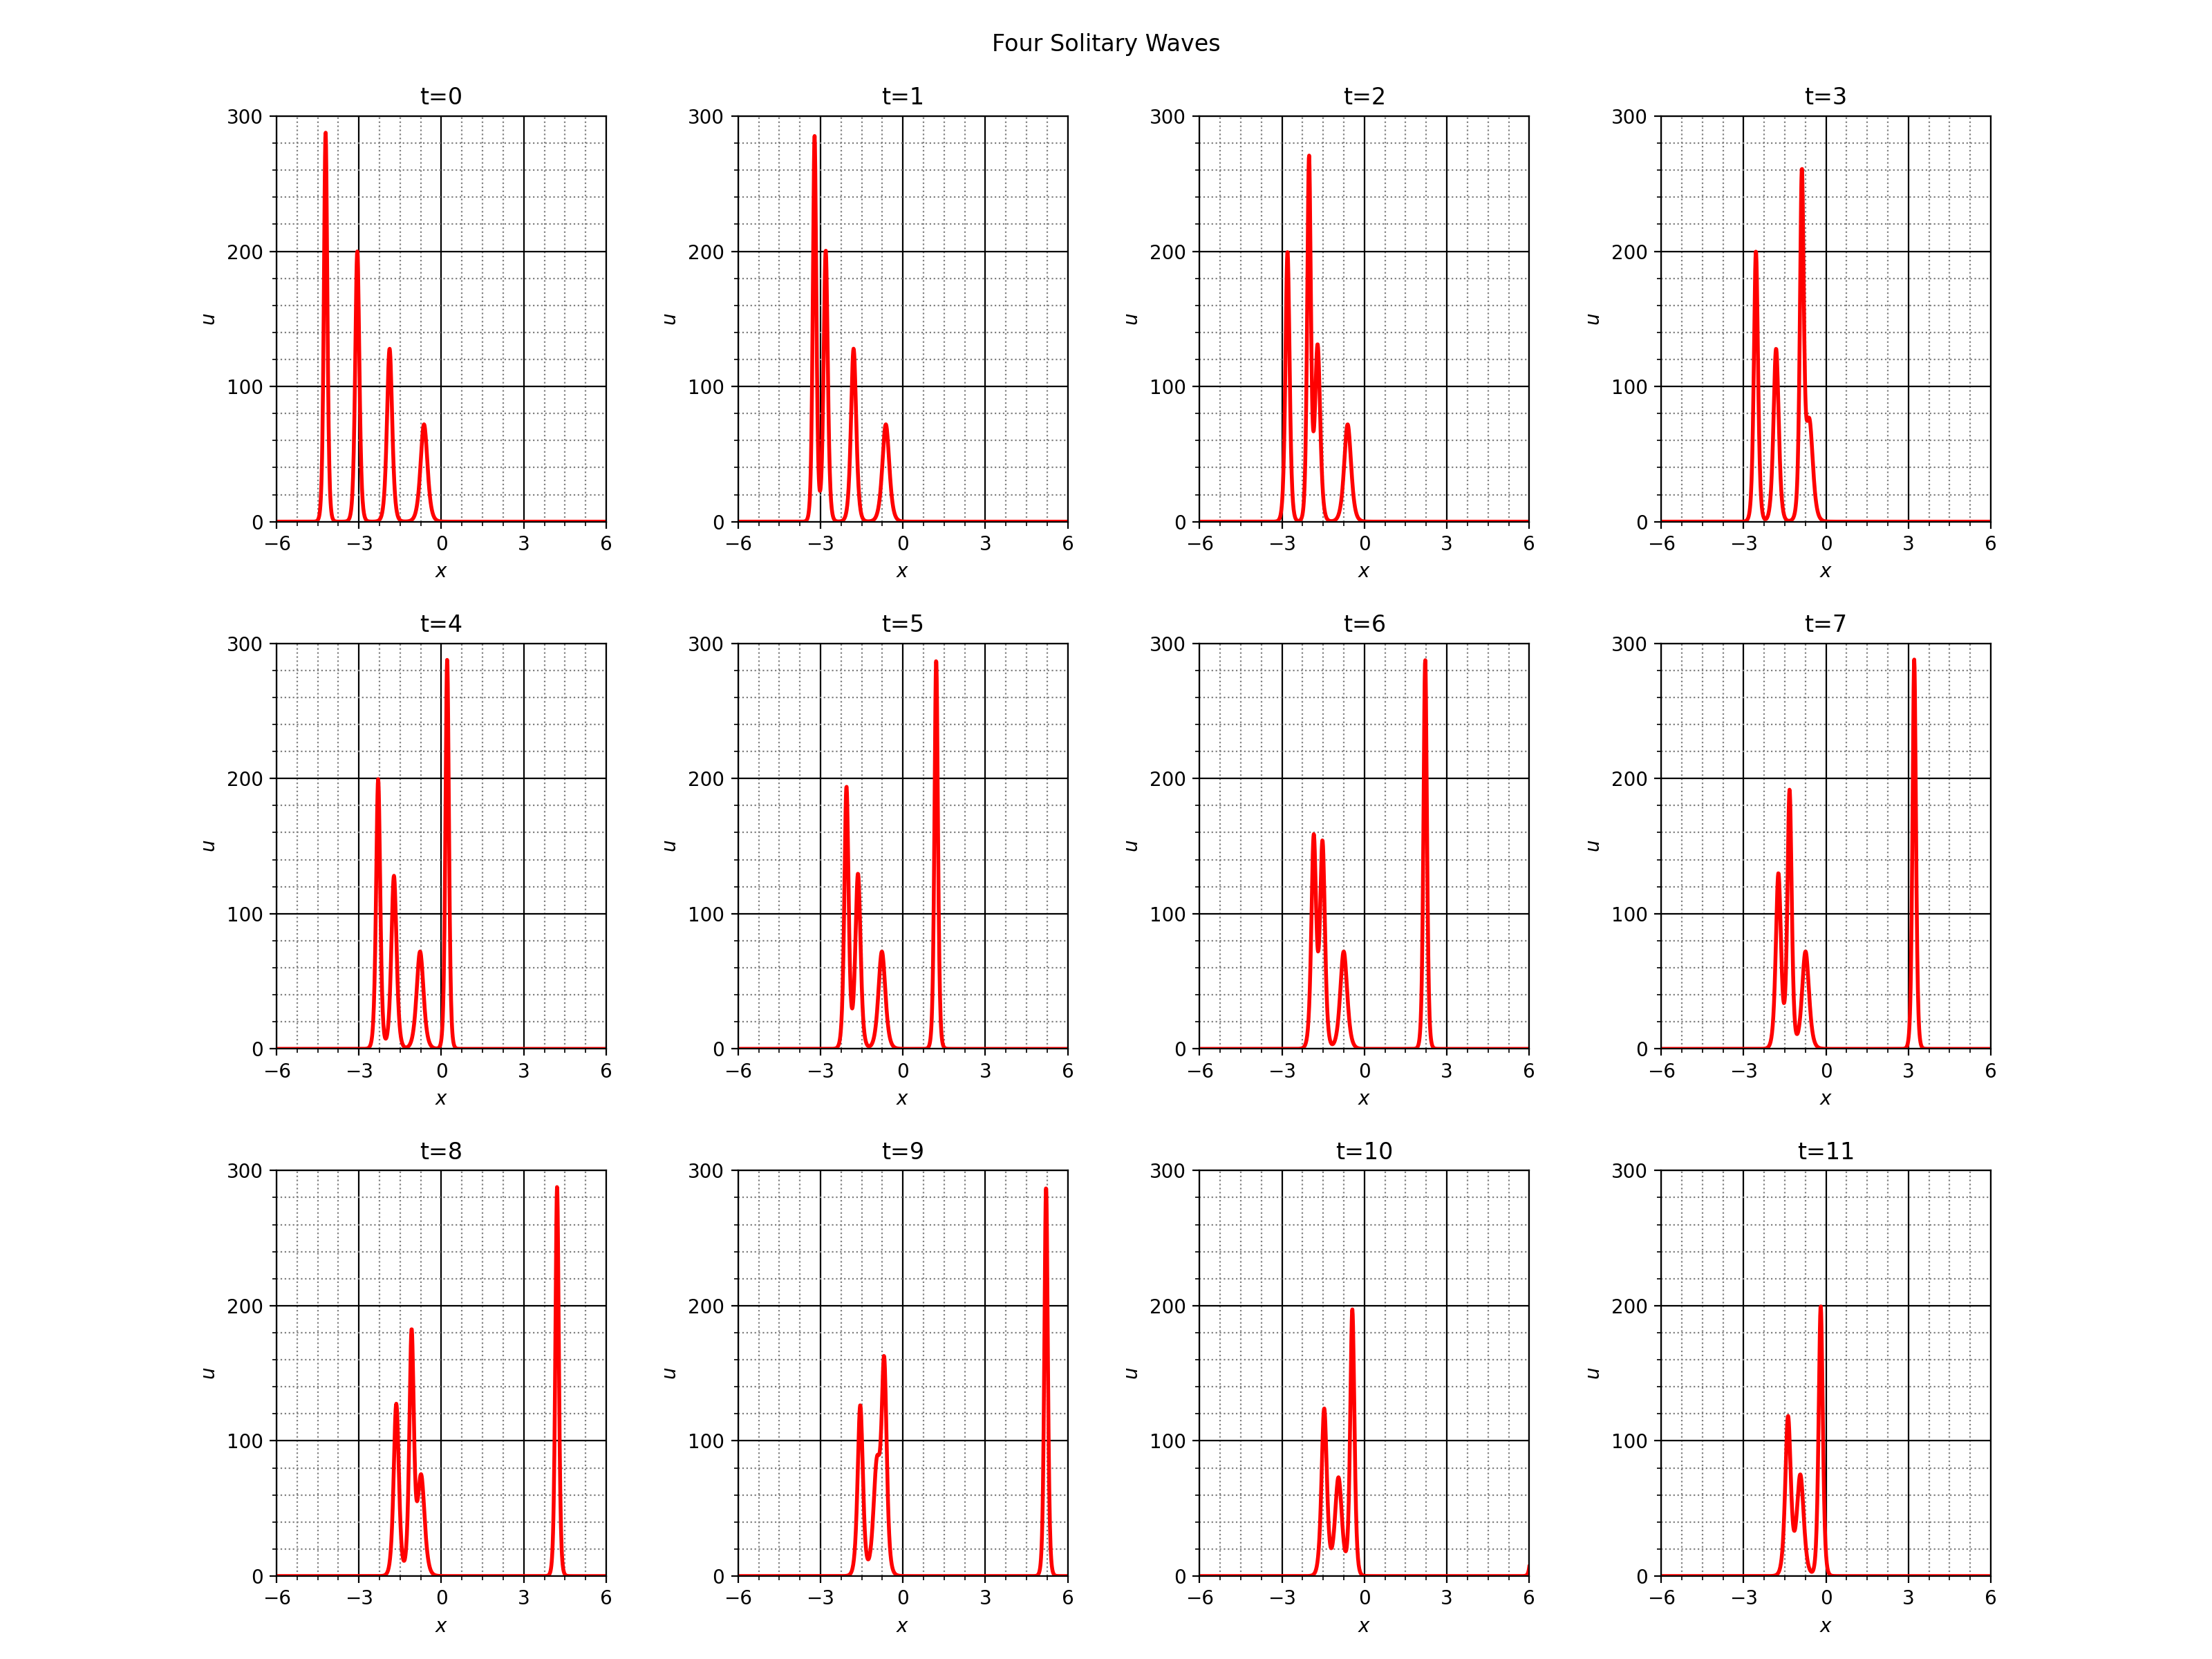
\includegraphics[width=190mm]{Figure_1.png}
  \caption{Решение при параметрах: $\varkappa_1 = 6,\varkappa_2 =8,\varkappa_3=10,\varkappa_4 = 12 $}
  \label{fig}
 \end{center}
\end{figure}


\end{document}
